%% Template for a preprint Letter or Article for submission
%% to the journal Nature.
%% Written by Peter Czoschke, 26 February 2004
%%

\documentclass{nature}

%% make sure you have the nature.cls and naturemag.bst files where
%% LaTeX can find them

\usepackage{graphicx}
\usepackage{siunitx}
\usepackage{url}
\usepackage{xcolor}
\usepackage{amsfonts, amsmath, amssymb}
\newcommand\ddfrac[2]{\frac{\displaystyle #1}{\displaystyle #2}}

\usepackage{hyperref}

\title{Global changes in oceanic mesoscale currents over the satellite altimetry record}

%\\ 2) Global significant observed trends of oceanic mesoscale processes\\ 3) Significant increase of oceanic mesoscale activity over the satellite record}

\author{Josu\'e Mart\'inez-Moreno$^1$, Andrew McC. Hogg$^1$, Matthew H. England$^2$, Navid C. Constantinou$^1$, Andrew E. Kiss$^1$  \& Adele K. Morrison$^1$}

%% macros
\newcommand{\KE}{\text{KE}}
\newcommand{\MKE}{\text{MKE}}
\newcommand{\TKE}{\text{TKE}}
\newcommand{\EKE}{\text{EKE}}
\newcommand{\SST}{\text{SST}}
\newcommand{\SSH}{\text{SSH}}

%% end of macros

\usepackage{multicol}

\spacing{2}

\begin{document}
	
\maketitle

\renewcommand{\thefootnote}{\roman{footnote}}

\begin{affiliations}
 \item Research School of Earth Sciences and ARC Centre of Excellence for Climate Extremes, Australian National University, Canberra, ACT, Australia
 \item Climate Change Research Centre and ARC Centre of Excellence for Climate Extremes, University of New South Wales, Sydney, NSW, Australia
\end{affiliations}

\begin{abstract}
	Oceanic mesoscale eddies play a profound role in mixing tracers such as heat, carbon, and nutrients, thereby regulating regional and global climate. Yet, it remains unclear how the eddy field has varied over the past few decades. Furthermore, climate model predictions generally do not resolve mesoscale eddies, which could limit their accuracy in simulating future climate change. Here we show a global statistically significant increase of ocean eddy activity using two independent observational datasets of surface mesoscale eddy variability, one estimates surface currents and the other is derived from sea surface temperature. Maps of mesoscale variability trends show heterogeneous patterns, with eddy-rich regions showing a significant increase of 2\% - 5\% per decade, while the tropical oceans show a decrease in mesoscale variability. This readjustment of the surface mesoscale ocean circulation has important implications for the exchange of heat and carbon between the ocean and atmosphere.
\end{abstract}

Changes in the climate system over recent decades have warmed the upper ocean and modified the wind stress, heat and freshwater fluxes that drive ocean circulation\cite{IPCC_2019_ocean,intergovernmental2007climate}. These changes have the capacity to modify the ocean circulation, including the overturning circulation\cite{Marshall_MOC_2017,Toggweiler_circulation_2008},  basin-scale gyres\cite{Yang_shift_2020,Sutton_basin_2007} and boundary currents\cite{Wu_warming_2012,Kwon_BC_atm_2010}. Changes in climate can also affect mesoscale processes, for example through changes in wind stress forcing over the Southern Ocean\cite{Hogg_Recent_2015}. The oceanic mesoscale incorporates motions that occur at spatial scales from approximately 10 to 100 km. These motions include both steady flows (e.g. jets and recirculations) and time-varying flows (e.g. meanders and coherent vortices). Generally, time-varying mesoscale flows are also referred to as eddies. Mesoscale eddies are ubiquitous in the global ocean and feed back onto all scales, from regional processes\cite{Radko_diapycnal_2004} up to the global meridional overturning circulation\cite{Marshall_MOC_2017}. Moreover, these eddies act to transport and mix tracers such as heat, salt, and nutrients\cite{Chelton_The_2011,Early_propagation_2011}. Thus, understanding the evolution of the mesoscale circulation is crucial to formulating better predictions of our changing oceans.

Kinetic energy ($\KE$) quantifies the magnitude of ocean currents\cite{Meredith_Sensitivity_2012,Hogg_Recent_2015,Busecke_mesoscale_2019,Hu_acceleration_2020}. Kinetic energy is proportional to the square of the velocity, and is commonly separated into the mean $\KE$ ($\MKE$; computed from the time-mean velocity field) and the $\KE$ of the time-varying velocity (known as the eddy kinetic energy; $\EKE$). The $\EKE$ is dominated by mesoscale variability and is a significant fraction of the total $\KE$\cite{Wyrtki_Eddy_1976, Chelton_Global_2007}. A recent study has inferred a global increase of $\KE$ anomaly from ocean reanalyses and Argo floats\cite{Hu_acceleration_2020}. However, these reanalyses and observations do not have the spatial resolution required to resolve the mesoscale field. Moreover, the ECCO ocean state-estimate shows a slight speed up of the currents, with a weak trend of surface kinetic energy\cite{Wunsch_speeding_2020}. In contrast, satellite observations resolve the mesoscale field at latitudes between 60$^\circ$S - 60$^\circ$N, and suggest that EKE in the Southern Ocean and Northeastern Pacific have a robust increasing trend\cite{Hogg_Recent_2015,Patara_Variability_2016,Martinez_TKE_2019,Ding_Increased_2017}. However, the global multi-decadal trends of mesoscale eddy activity from satellite observations are yet to be quantified.

Mesoscale flows have a footprint in both sea surface height ($\SSH$) and sea surface temperature ($\SST$). EKE can be directly inferred from SSH via geostrophy, and mesoscale eddies act to strain and shear the temperature field, meaning that regions of high EKE are associated with strong mesoscale SST gradients. Therefore, observed SST gradients can be considered a proxy of mesoscale eddies\cite{Yuan_eddy_induced_2017,Castellani_SST_identif_2006,Holladay_mesoscale_1975}.

In this study we examine the evolution of mesoscale eddies using satellite observations of $\SSH$ and $\SST$ over the satellite altimetry record (1993~-~2020). We use two independent datasets, namely AVISO+ $\SSH$ and NOAA optimum interpolated sea surface temperature (OISST v2.1)\cite{Banzon_OISST_2020}, to estimate $\EKE$ and $\SST$ gradients respectively (see Methods). These fields are then temporally smoothed using a running average of 12 months to eliminate the seasonal cycle. The trends and the significance of each field are computed using a linear regression and a modified Mann--Kendall test\cite{Sheng_MK_2004} (see Methods for further details). Mesoscale variability is spatially heterogeneous; thus we explore the trends of mesoscale eddies both globally and regionally.

\subsection{Global mesoscale eddy trends}\mbox{}\vspace{-1.5em}

Over the last three decades, ocean thermal expansion and melting of land ice have led to an increase of $\SSH$\cite{IPCC_2019_ocean,Polito_SST_trends_2008} (Fig.~\ref{fig:global_trends}a). This SSH increase can be observed in all ocean basins, but there is also regional variability (Fig.~\ref{fig:global_trends}b). SSH gradients are proportional to the surface geostrophic flow, from which we can compute velocity anomalies and eddy kinetic energy (see Methods). The time-mean $\EKE$ highlights eddy-rich regions including boundary currents and their extensions, the Antarctic Circumpolar Current (ACC), and the equatorial band (Fig.~\ref{fig:global_trends}d). These oceanic eddy-rich regions show statistically significant trends over the satellite altimetry record 1993-2020 (Fig.~\ref{fig:global_trends}f), which suggest a regional long-term adjustment of the ocean mesoscale eddy field. Moreover, the global surface area-integrated $\EKE$ has a positive trend of $\sim$1.2\% per decade (0.09 $\pm$ 0.04 PJ m$^{-1}$ decade$^{-1}$; Fig.~\ref{fig:basin_trends}c; statistically significant at the 95\% confidence level). The spatial structure of $\EKE$ trends is highly heterogeneous, although its zonal average shows significant net tendencies, with increasing trends observed polewards of 25$^\circ$S and 40$^\circ$N (Fig.~\ref{fig:global_trends}e,f). A strengthening of the EKE field is a direct indication of an increase in mesoscale currents.

Sea surface temperature is an independent dataset relative to SSH, but is also influenced by mesoscale eddies and has better temporal and spatial resolution than $\SSH$. $\SST$ has increased on multi-decadal timescales due to climate change\cite{Cane_sst_trends_1997,Ruela_SST_2020} (Fig.~\ref{fig:global_sst_ssh_trends}a), with a heterogeneous global spatial pattern modulated by interdecadal climate variability\cite{Cane_SST_trends_2997} (Fig.~\ref{fig:global_sst_ssh_trends}b).
The time-mean $\SST$ gradients again highlight eddy-rich regions, such as boundary currents, their extensions, and the ACC (Fig.~\ref{fig:global_sst_ssh_trends}d). These regions with large $\SST$ gradients also exhibit some of the largest positive $\SST$ gradient trends, while the subtropical gyres and the tropics mostly exhibit a decreasing trend (Fig.~\ref{fig:global_sst_ssh_trends}e,f). The global area-integrated $\SST$ gradient magnitude has increased at a rate of 3.9 $\pm$ 1.33 $ \mathrm{\times10}^{6}\ ^\circ \mathrm{C}$ m decade$^{-1}$ (Fig.~\ref{fig:basin_trends}e) or 0.2\% per decade (95\% confidence level) relative to the global time-mean area-integrated $\SST$ gradient magnitude (1.7 $\mathrm{\times10}^{9}\ ^\circ \mathrm{C}$ m). Moreover, SST gradients are enhanced by stretching and straining due to mesoscale eddies. Further analysis shows that mesoscale $\SST$ gradients (Extended Data Fig.~3; length-scales smaller than 3$^\circ$; see Methods) dominate the observed trends, increasing at a rate of 5.37 $\pm$ 0.94 $ \mathrm{\times10}^{6}\ ^\circ \mathrm{C}$ m decade $^{-1}$ (0.4\% per decade; statistically significant at the 95\% confidence level). This analysis confirms that the observed $\SST$ gradient trends are a consequence of the mesoscale eddy field stirring the temperature field.

Eddy kinetic energy and mesoscale SST gradients show analogous spatial and temporal responses in the boundary currents and their extensions, the ACC and the tropics. Note that eddy-rich regions such as the Kuroshio Current, the Agulhas retroflection, the Gulf Stream, and the East Australian Current show large changes in mesoscale $\SST$ gradients co-located with some of the largest $\EKE$ changes (Fig.~\ref{fig:WBC_regional_small_scale_SST_grad}). Even though these fields do not match perfectly, we quantified the areas of same-sign trend for each of these four regions (Extended Data Fig.~4). We find that the increasing and decreasing trends of $\SST$ and $\EKE$ match to a good extent for the Kuroshio Current, the Agulhas retroflection, and the East Australian Current (61\% - 65\% of same-sign area agreement). The spatial patterns of these independent satellite products further suggest an intrinsic response of the mesoscale eddy field to a changing and variable climate.

\subsection{Spatial patterns of ocean mesoscale trends}\mbox{}\vspace{-1.5em}

Eddy kinetic energy and mesoscale $\SST$ gradient trends both indicate a net strengthening of the global mesoscale activity. However, both datasets reveal heterogeneous patterns of increasing and decreasing trends. Thus, to further understand the spatial variability, we first focus our analysis on individual area-integrated regions: namely, the Southern Ocean (by which we mean south of 35$^\circ$S), and the Pacific, Indian, and Atlantic Oceans north of 35$^\circ$S (Fig.~\ref{fig:basin_trends}d). This analysis reveals that the Southern Ocean and the Pacific Ocean are, to a large extent, responsible for the global area-integrated trends and variations of $\EKE$ and mesoscale $\SST$ gradients; the trends in the Indian and Atlantic Oceans are in contrast much smaller (Fig.~\ref{fig:basin_trends}a,b). The Southern Ocean shows a statistically significant increase for both the $\EKE$ and $\SST$ gradient, where the observed changes have been attributed to the strengthening of the wind stress since the early 1990s\cite{Hogg_Recent_2015}. The Pacific Ocean $\SST$ gradient decreases significantly, with the $\EKE$ signal also decreasing; albeit below the 95\% significance level (Fig.~\ref{fig:basin_trends}c,e). The large uncertainty in the Pacific $\EKE$ trend (orange error bars in Fig.~\ref{fig:basin_trends}c) is a consequence of the pulses in the time series during 1997 and 2015, both being El Ni\~no onset years. These large anomalous interannual signals dominate the uncertainty of the global $\EKE$ trend.

El Ni\~no events are associated with a strengthening of the  North Equatorial Countercurrent and the northern branch of the South Equatorial Current; particularly during extreme eastern Pacific El Ni\~nos, such as those which occurred during 1997-1998 and 2015-2016\cite{Wang_ENSO_2013} (gray bars in Fig.~\ref{fig:basin_trends}a,b). During such El Ni\~no events, the equatorial currents generate significant transient circulation anomalies that extend over the equatorial band (9$^\circ$N - 9$^\circ$S). After a scale decomposition of the velocities, we observe that these $\EKE$ pulses correspond to features located within the equatorial band and have scales larger than the typical mesoscale eddy size\cite{Chelton_The_2011} (approximately 10 to 100 km; see Methods;  Extended Data Fig.~5a,c). Thus, equatorial currents during El Ni\~no events modulate the equatorial $\EKE$ response and the strong interannual variability conceals $\EKE$ trends over the equatorial region.

To further investigate the effect of El Ni\~no events on the mesoscale, we remove the equatorial regions (9$^\circ$S--9$^\circ$N) and repeat the global trend analysis for $\EKE$ and $\SST$ gradients. The global area-integrated extra-tropical $\EKE$ and $\SST$ gradient trends increase, while the corresponding relative uncertainty decreases; namely, $\EKE$ trends are $1.8\% \pm 0.25 \%$ per decade and mesoscale $\SST$ gradients trends are $1.6\% \pm 0.09 \%$ per decade (see striped bars in Fig.~\ref{fig:basin_trends}c,e); both significant at the 95\% confidence level. It is thus clear that mesoscale activity in the Pacific, and particularly in the equatorial region, is strongly influenced by interannual variability. 

\subsection{Eddy-rich regions become richer}\mbox{}\vspace{-1.5em}

The observed changes in $\EKE$ and $\SST$ of whole ocean basins integrate over large heterogeneous regions with opposing trends. For example, the Pacific Ocean aggregates the strengthening of the equatorial currents in the equatorial Pacific Ocean during El Ni\~no events, boundary currents, and the broader-scale oceanic gyres. These dynamical regions are not unique to the Pacific Ocean; the Atlantic and Indian basins also span diverse dynamical regions. Therefore, we further decompose the ocean into dynamical regions (Fig.~\ref{fig:process_trends}d): namely, (1) the Antarctic Circumpolar Current (ACC) and surrounds, (2) the boundary currents and their extensions, (3) the equatorial regions, and (4) the subtropical ocean gyres (see Methods for dynamical region definitions). The remaining regions are aggregated into a fifth group. We then investigate the variability and trends within each of these dynamical sub-regions.

Globally, there is a significant increase of $\EKE$ and $\SST$ gradients, however, each dynamical region shows a different response (Fig.~\ref{fig:process_trends}). For example, the ACC region shows a significant increase in both $\EKE$ and $\SST$ gradients at rates of 5.1\% and 3\% per decade (Fig.~\ref{fig:process_trends}c,e), consistent with an increase in eddy activity with strengthening wind stress, as demonstrated in previous studies\cite{Meredith_Sensitivity_2012,Hogg_Recent_2015,Martinez_TKE_2019}. Boundary currents and their extensions collectively show a similar net response, in which $\EKE$ and $\SST$ gradients both increase at rates of 2.5\% and 8.1\% per decade respectively. Individually, $\SST$ gradients increase in all boundary currents, however $\EKE$ in the Agulhas retroflection, the East Australian Current, the Leeuwin Current, and the Malvinas Current have significantly increased, but the Gulf Stream and the Kuroshio Current do not show a significant net strengthening\cite{Ezer_Gulf_Stream_2013,Uchida_Kuroshio_2008}(Extended Data Fig.~6); instead, regions of increase and decrease tend to cancel each other out in an area-integral. This cancellation is particularly evident for the Kuroshio Current (Fig.~\ref{fig:global_trends}f and  Extended Data Fig.~6b). The response seen in the Gulf Stream and Kuroshio Current is consistent a poleward shift in these currents\cite{Wu_shift_2020,Yang_intensification_2016, Wu_warming_2012} and a readjustment to climate modes\cite{Piecuch_Fcurrent_2020}. Note that a poleward shift cannot be captured by our static climatological definition of the boundary currents regions (see Methods). Thus,  a shift of the boundary currents will result in an increase of $\EKE$ and $\SST$ gradients outside our dynamical definitions (i.e. in regions poleward of the boundary currents and ocean gyres; white regions in Fig.~\ref{fig:process_trends}d). The observed strengthening of these remaining regions is comparable to that of the ACC, and suggests a poleward shift of the boundary currents, particularly in the Northern Hemisphere. 
%\ref{fig:individual_boundary_currents}

The equatorial and subtropical gyre regions exhibit statistically significant negative $\SST$ gradient trends, and statistically non-significant negative $\EKE$ trends (Fig.~\ref{fig:process_trends}), suggesting a reduction of the mesoscale eddy variability of the equatorial region and the interior of the subtropical gyres (Fig.~\ref{fig:global_sst_ssh_trends}). The equatorial region is dominated by interannual variability, where large changes corresponding to El Ni\~no events occur in both the $\EKE$ and $\SST$ gradient time series. The significant decrease of $\SST$ gradients in the subtropical gyres could result from the displacement of the extratropical atmospheric circulation\cite{Saenko_response_2005,Gupta_changes_2009} and the expansion of the tropics\cite{Seidel_widening_2007}.  The decreasing SST gradient trends in the tropics could be due to a homogenization of the tropical surface $\SST$ gradients. In the future, the $\SST$ gradients induced by mesoscale stirring are expected to reduce as the surface ocean becomes more thermally homogeneous. However, a longer record is required to separate the mesoscale response from interannual-decadal climate variability. 

We have analyzed the available satellite altimetry record of $\SSH$ and $\SST$ to reveal a significant global intensification of the mesoscale eddy field over the satellite record. While the observed global surface percentage increases per decade may seem small ($\sim0.5\%$ per decade), like ocean heat content and sea-level trends, even small fractions of a percentage change correspond to a large energy perturbation of the earth system. For example, if we assume that the mesoscale flow extends vertically to around 500 m depth (a reasonable assumption given the vertical structure of the gravest mode\cite{Lama_Vmodes_2016}), then the observed $\EKE$ trends integrated over 500 m imply a significant increase of 0.7\% in the global volume-integrated mesoscale energy budget (13 $\times10^{18}$ J \cite{Wunsch_energy_2004}) over the satellite altimetry record after removing the El Ni\~no signal (Extended Data Fig.~5b). This percentage is equivalent to 0.9$\times10^{17}$ J, the same order of magnitude as the global internal tide energy budget (1 $\times10^{17}$ J \cite{Wunsch_energy_2004}). Eddy kinetic energy in eddy-rich regions, such as boundary current extensions and the ACC, exhibit even larger significant strengthening of 2\% and 5\%, respectively (see Fig. 5). Increased mesoscale activity observed in both $\SST$ and mesoscale $\SST$ gradients is most apparent in regions where eddies are already strong. These eddy-rich regions are critical for carbon and heat uptake by the ocean\cite{Foppert_Eddy_2017,Gnanadesikan_carbon_uptake_2015}, and they are known to be sensitive to climate modes that are readjusting in a changing climate; for example, the strengthening of the westerly winds\cite{Hogg_Recent_2015} linked to recent increasing trends in the Southern Annular Mode\cite{Nerilie_SAM_2014,Gillett_SAM_2013}. With ongoing future projected changes in the westerly wind belt, it is expected that mesoscale activity in the southern hemisphere boundary currents and the ACC will continue to increase over the coming decades. Current generation models used for climate projections (CMIP6) do not generally resolve mesoscale eddies\cite{Haarsma_CMIP6_2016}; thus, important climatic adjustments driven by changes in the eddy field are likely to be missing from these climate projections.

The mesoscale evolution described here cannot be captured by coarse-resolution reanalysis products and sparse Argo float observations, as previously used in other studies\cite{Hu_acceleration_2020}.
Here we have used eddy-permitting satellite observations to reveal a potential decrease in $\EKE$ over the tropics, while reanalysis products suggest the tropics is where $\KE$ anomalies have increased the most\cite{Hu_acceleration_2020}. The $\KE$ anomaly differs from $\EKE$ because it contains the time-mean flow in addition to the time-varying components. The source of differences between Hu \textit{et al.}, (2020)\cite{Hu_acceleration_2020} and our results can be assessed by an analysis of the ocean $\KE$ anomaly using satellite observations. The $\KE$ anomaly trends are almost identical to the $\EKE$ trends presented above (compare Fig.~\ref{fig:global_trends} and  Extended Data Fig.~7), yet strikingly different from those obtained by Hu \textit{et al.}, (2020) (their Fig 2a).
This suggests that the difference between our results and those of Hu \textit{et al.}, (2020) arises from the inability of reanalyses and the Argo dataset to resolve the mesoscale, due to coarse-resolution and sparse sampling, rather than from the definition of the $\KE$ anomaly. An alternative explanation of the differences between our study and Hu \textit{et al.}, (2020) could arise from the KE anomaly trends in Hu \textit{et al.}, (2020) being depth-integrated (0-2000 m), while our EKE calculations are derived solely from surface diagnostics. In addition, as we have demonstrated, the tropics are strongly influenced by interannual variability (e.g. El Niño), and yet the $\KE$ time-series from coarse reanalysis data does not detect the two extreme El Niño events observed in the satellite record. Thus, data resolution and/or subsurface ocean dynamics are the likely causes of the discrepancy between our eddy-permitting analysis and the results from prior work using reanalysis products\cite{Hu_acceleration_2020}.
%\ref{fig:global_trends_asper_hu}

There are several possible causes of the observed trends in mesoscale activity including (1) changes in winds (wind curl, wind stress), (2) changes in stratification, and (3) changes in large-scale horizontal temperature gradients. These forcing agents can impact the eddy activity via a combination of processes, e.g., non-local intensification of winds, outcropping and tilting of isopycnals, and strengthening of baroclinic instability. Atmospheric reanalyses show distinct and inconsistent wind stress trend patterns, while records of \textit{in situ} measurements of isopycnal tilt and baroclinic growth rate are too short and too sparse to provide evidence of a dynamical mechanism driving the observed increase in eddy activity. Thus, longer observational records with higher temporal and spatial frequency are required to better understand the increase in EKE observed from satellites. In addition, as discussed above, trends computed from coarse-resolution ocean reanalysis products\cite{Hu_acceleration_2020} with parameterized mesoscale eddies differ significantly from the mesoscale trends we detect from eddy-resolving satellite altimetry. Hence, an in-depth analysis of the dynamics leading to the observed mesoscale eddy evolution should be explored in more detail using truly eddy-resolving global ocean models or eddy-resolving reanalysis products.

Our study has documented a major global-scale reorganization of the ocean's mesoscale kinetic energy observed over the past three decades. These observed adjustments in the mesoscale field have the potential to affect ocean circulation at regional and global scales, and to modify the transport and redistribution of tracers, such as heat, carbon, and nutrients. Our findings thus have major implications for ocean readjustment to a changing climate, as the enhancement of the mesoscale ocean currents may feed back on the sequestration of anthropogenic heat and carbon into the ocean. 

\bibliographystyle{naturemag}
\bibliography{biblio}

\subsection{Acknowledgments}\mbox{}\vspace{-1.5em}

We thank Ryan Holmes for clarifying the equatorial response of El Ni\~no events during 1997-1998 and 2015-2016.  We thank the reviewers for their insightful comments and suggestions. The satellite altimetry products were produced by Ssalto/Duacs and distributed by AVISO+, with support from CNES (\url{https://www.aviso. altimetry.fr/en/data/products/sea‐surface‐height‐products/global/gridded‐sea‐level‐heights‐and‐derived‐ variables.html}). J. M.‐M. was supported by the Consejo Nacional de Ciencia y Tecnología (CONACYT), Mexico funding. M.H.E. was supported by the Centre for Southern Hemisphere Oceans Research (CSHOR), a joint research centre between QNLM, CSIRO, UNSW and UTAS. A. K. M. was supported by the Australian Research Council DECRA Fellowship DE170100184. Analyses were undertaken on the National Computational Infrastructure in Canberra, Australia, which is supported by the Australian Commonwealth Government. 

\subsection{Author contributions}\mbox{}\vspace{-1.5em}

J.M.M, A.McC.H. and M.H.E. conceived the study. J.M.M. conducted the analyses. All authors contributed to interpretation, writing and revision of the manuscript.

\newpage

\spacing{1}

\begin{figure}
    \centering
	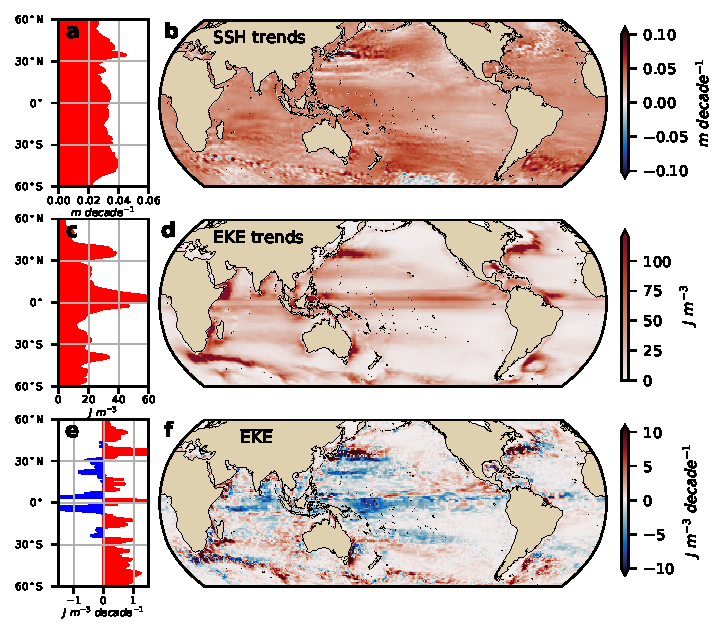
\includegraphics[width=\textwidth]{./figures/global_trend_WBC_GW_nsignif.pdf}\\
	\caption{\textbf{Sea surface height ($\SSH$) trend, mean surface eddy kinetic energy ($\EKE$) and surface eddy kinetic energy trend between 1993-2020} (a) Zonally averaged $\SSH$ trend; (b) map of $\SSH$ trend (92.1\% of area is statistically significant above the 95\% confidence level; for spatial distribution refer to Extended Data Fig.~1a); (c) zonally averaged mean $\EKE$; (d) map of mean $\EKE$; (e) zonally averaged $\EKE$ trend; (f) map of $\EKE$ trend (55.4\% of area is statistically significant above the 95\% confidence level; see Extended Data Fig.~1b). \label{fig:global_trends}}
\end{figure}
%\ref{fig:global_significance_trends}

\begin{figure}
    \centering
	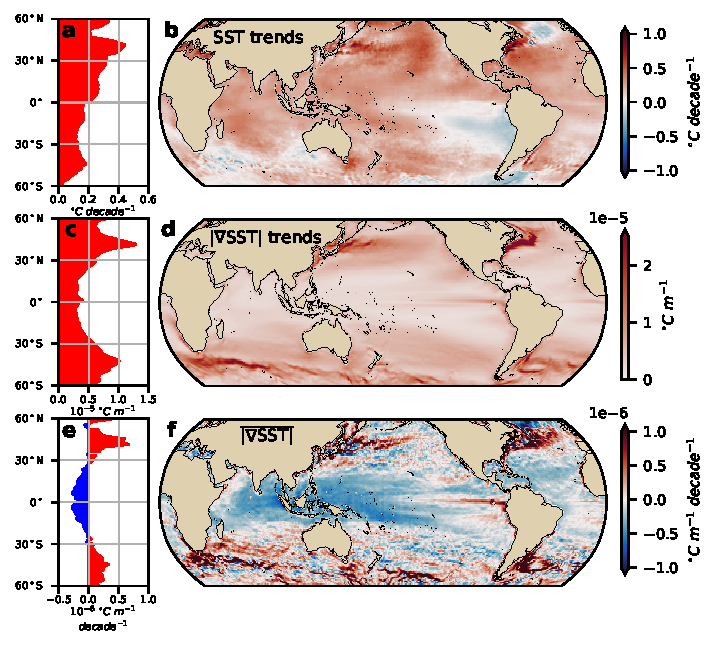
\includegraphics[width=\textwidth]{./figures/global_SST_SST_grad_SSH_trends.pdf}\\
	\caption{\textbf{Sea surface temperature ($\SST$) trends, mean $\SST$ gradient magnitude, and $\SST$ gradient magnitude trends between 1993-2020.} (a) Zonally averaged $\SST$ trend; (b) map of $\SST$ trend (76.7\% of area is statistically significant above the 95\% confidence level; for the spatial distribution refer to Extended Data Fig.~1c); (c) zonally averaged time-mean of $\SST$ gradient magnitude; (d) map of time-mean of $\SST$ gradient magnitude; (e) zonally averaged $\SST$ gradient magnitude trend; (f) map of $\SST$ gradient magnitude trends (81.6\% of area is statistically significant above the 95\% confidence level; see Extended Data Fig.~1d). Note that the spatial pattern of $\SST$ gradient maps is independent of the temporal extent of the $\SST$ gradient record used to compute $\SST$ gradient trends (Extended Data Fig.~2). \label{fig:global_sst_ssh_trends}}
\end{figure}
%\ref{fig:global_significance_trends}

\begin{figure}
    \centering
	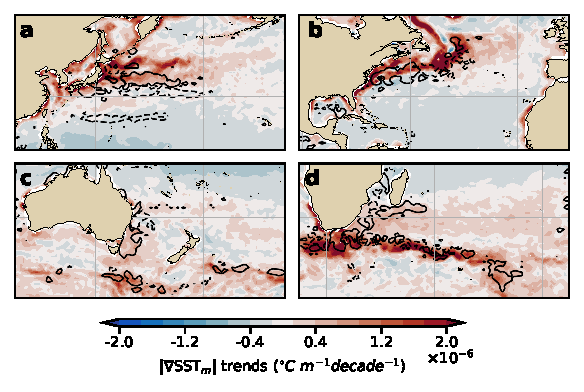
\includegraphics[width=\textwidth]{./figures/global_SST_small_scales_tke_trends.pdf}\\
	\caption{\textbf{Regional maps of mesoscale $\SST$ gradient magnitude trends and surface $\EKE$ trends}.  (a) Kuroshio Current; (b) Gulf Stream; (c) East Australian Current; (d) Agulhas retroflection. In all panels, mesoscale SST gradient magnitude trends are shown by the background color, solid contours show positive $\EKE$ trends and dashed contours show negative $\EKE$ trends (contours of $\pm 5\ J\ m^{-3}\ decade^{-1} $).  \label{fig:WBC_regional_small_scale_SST_grad}}
\end{figure}

\begin{figure}
    \centering
	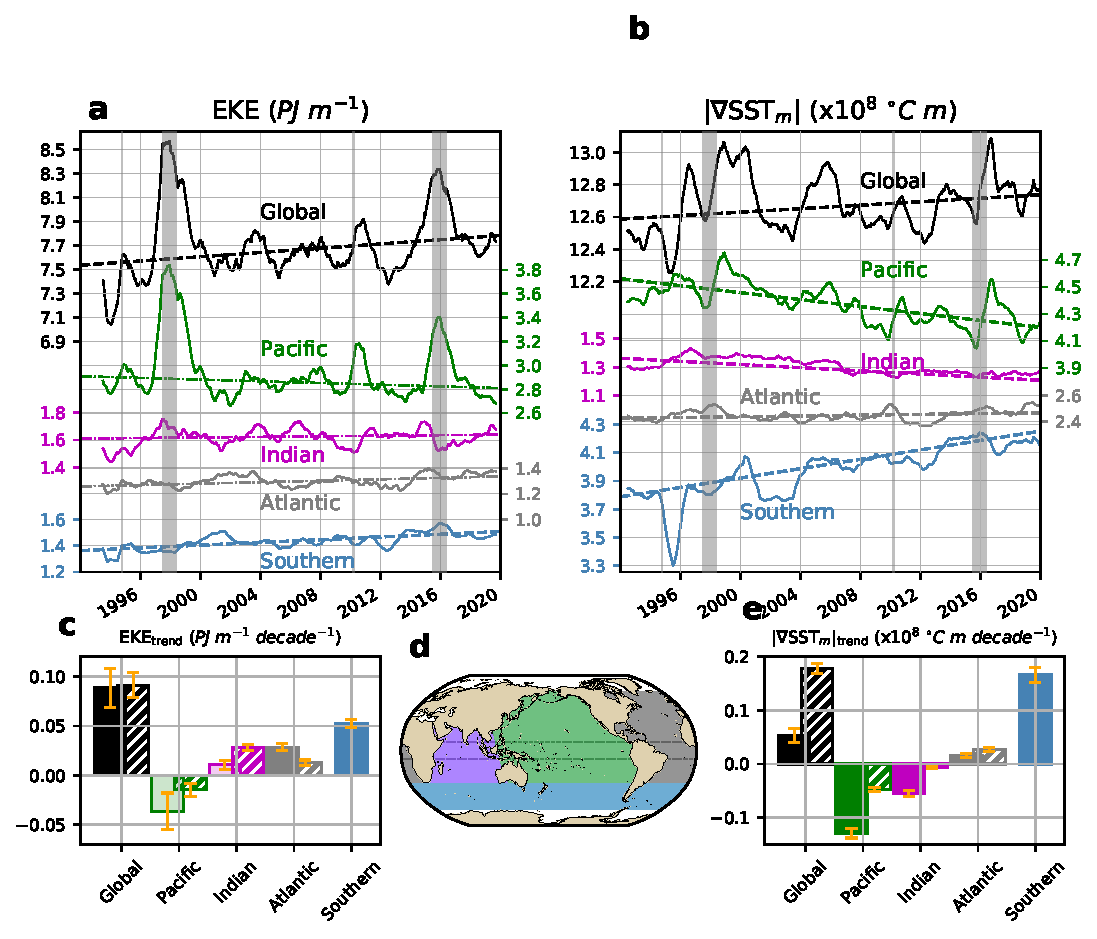
\includegraphics[width=1\textwidth]{./figures/global_basin_trends_FV.pdf}\\
	\caption{\textbf{Time-series and linear trends of area integrated surface $\EKE$ and mesoscale $\SST$ gradient magnitudes over various ocean basins.} Global (solid black), Southern (blue), Indian (magenta), Pacific (green), and Atlantic Oceans (gray) and each region separately without the equatorial region (striped bars). (a) Surface $\EKE$  time series. (b) mesoscale $\SST$ gradient magnitude time series. In panels (a) and (b), solid curves denote 12-month running averages for each basin, dashed lines correspond to statistically significant time-series trends, dashed-dotted lines show statistically insignificant time-series trends, and vertical gray bars indicate El Ni\~no events (above the 90th percentile of MEI.v2\cite{Wolter_ENSO_1998}). Note that the y axis is discontinuous in panels (a) and (b). (c) Linear $\EKE$ trends for each basin. (d) Ocean basins; equatorial region (9$^\circ$S--9$^\circ$N) is marked by the dashed lines. (e) Linear mesoscale $\SST$ gradient trends. In panels (c) and (e), standard errors are shown with orange bars and statistically significant trends (above the 95\% confidence level) are solid bars while non-significant trends are translucent. \label{fig:basin_trends}}
\end{figure}

\begin{figure}
    \centering
	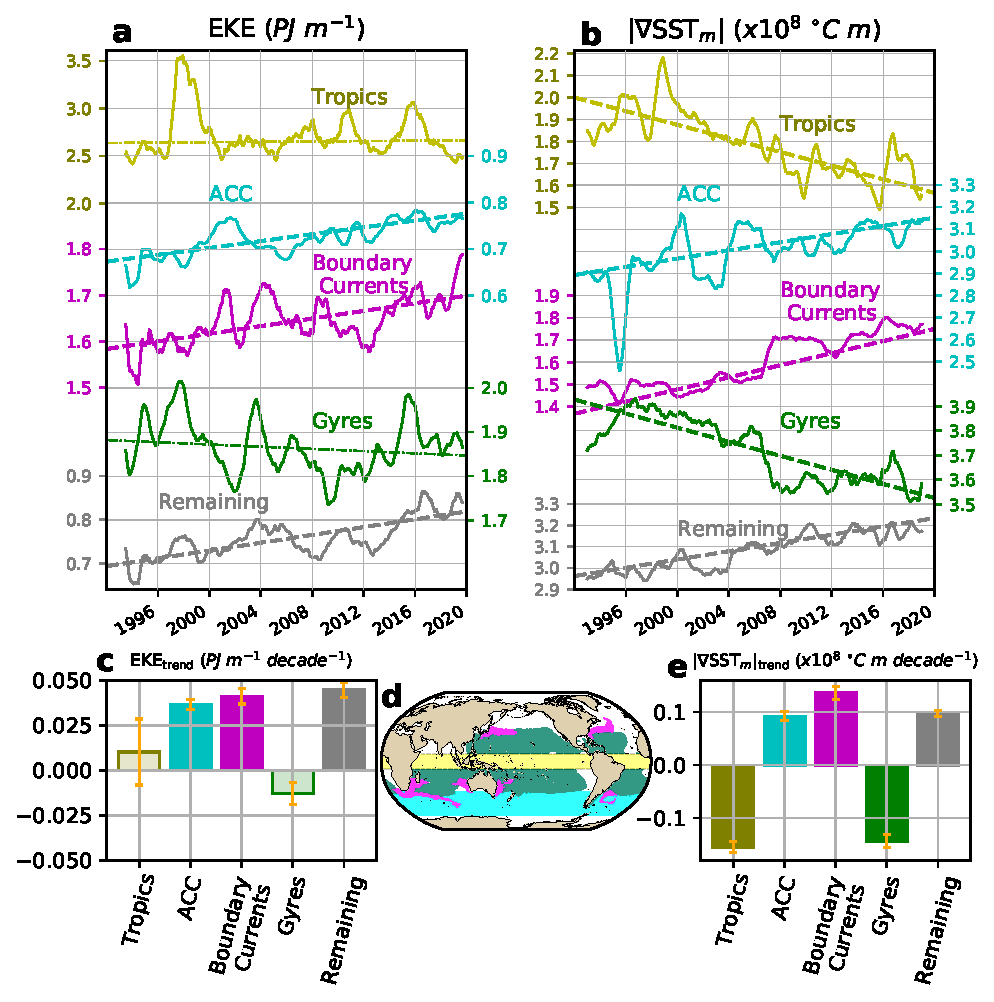
\includegraphics[width=0.90\textwidth]{./figures/global_processes_trends_FV.pdf}\\
	\caption{
	\textbf{Time-series and linear trends of integrated surface $\EKE$ and mesoscale $\SST$ gradient magnitudes over dynamical regions.} Global ocean (black), Tropics (yellow), Antarctic Circumpolar Current (cyan), boundary currents and their extensions (magenta), subtropical ocean gyres (green) and the rest (gray). (a) Surface $\EKE$ time-series. (b) mesoscale $\SST$ gradient magnitude time-series. In panels (a) and (b), solid color curves are 12-month running for each region, dashed lines correspond to statistically significant time-series trends, and dashed-dotted lines show insignificant time-series trends. (c) Linear $\EKE$ trends for each dynamical region. (d) Definition of ocean regions. (e) Linear mesoscale $\SST$ gradient trends. Note that in panel (a) the top curve that corresponds to the Tropics has a different scale than the rest.
	In panels (c) and (e), standard errors are shown with orange bars and statistically significant trends (above the 95\% confidence level) are solid bars while non-significant trends are translucent. \label{fig:process_trends}
	}
\end{figure}

\newpage

\spacing{2}
\section*{Methods}

\subsection{Observational products}\mbox{}\vspace{-1.5em}

The data used in this study includes sea surface height, geostrophic velocities, and sea surface temperature. The Archiving, Validation and Interpretation of Satellite Oceanographic data (AVISO+) gridded multi-mission sea surface height and geostrophic velocities have a horizontal resolution of 1/4$^\circ$ (although the effective resolution may be coarser in some regions \cite{Chelton_The_2011}). Currents within the equatorial region (5$^\circ S$-5$^\circ N$) are estimated using an equatorial $\beta$-plane approximation of
the geostrophic equations\cite{Lagerloef_velocities_1999}. National Oceanic and Atmospheric Administration - Optimum Interpolation Sea Surface Temperature (NOAA-OISST) has a horizontal resolution of 1/4$^\circ$\cite{Banzon_OISST_2020}. This dataset is constructed by combining observations from different products (e.g. satellites, ships, buoys, and Argo floats).

These datasets have a quasi-global coverage (65$^\circ$S--65$^\circ$N) and span 27 years, from January 1993 to March 2020. The SST product is available for a longer duration, but we only analyze the period of overlap with the AVISO+ record (see Extended Data Fig.~2). Anomalies were computed with respect to the record's climatology. We have verified that using a different period for defining the climatology does not change the observed trends in the anomaly fields. We have also verified through wavelet analysis of the time-series at individual points that there is no evidence that steps in the record occurred due to improved technology in satellite missions and oceanographic observations.

\subsection{Kinetic energy decomposition}\mbox{}\vspace{-1.5em}

Kinetic energy (KE) density is decomposed into the energy density contained by the steady flow (time-mean) and that contained by the transient flow (time-varying). In other words, the surface geostrophic velocity components are split using a Reynolds decomposition into their time-mean ($\overline{u}$, $\overline{v}$) and time-varying components ($u'=u-\overline{u}$, $v'=v-\overline{v}$), with bars denoting time-averages over the whole record. The terms $u'$ and $v'$ are the anomalies of the surface geostrophic velocities provided by AVISO+, which are proportional to the AVISO+ $\SSH$ gradients (via the geostrophic approximation and equatorial beta-plane approximation). The KE is, therefore, decomposed as:
\begin{linenomath*}
\begin{equation}
	\underbrace{\frac{1}{2}\rho_0\left(u^2 + v^2\right)}_{\KE}  = \underbrace{\frac{1}{2}\rho_0\left(u'^2 + v'^2\right)}_{\EKE}+\underbrace{\frac{1}{2}\rho_0\left(\overline{u}^2 + \overline{v}^2 \right)}_{\MKE} + \underbrace{\vphantom{\frac1{2}}\rho_0(\overline{u}u'+\overline{v}v')}_{\textrm{Cross terms}},
\end{equation}
\end{linenomath*}

where we approximate the density of the seawater by the constant $\rho_0 = $ 1025 $kg\,m^{-3}$. The energy contained in the time-varying component of the flow is known as the eddy kinetic energy ($\EKE$), while the mean kinetic energy ($\MKE$) is the energy of the time-mean flow.

Maps of $\EKE$ in this study correspond to the the time-mean $\EKE$, defined as
\begin{linenomath*}
\begin{equation}
	\overline{\EKE}(x,y) =  \overline{\frac{1}{2} \rho_0 (u'^2 + v'^2)},
\end{equation}
\end{linenomath*}
% where $A_g$ refers to the area of each grid cell.
where the units of $\overline{\EKE}(x,y)$ are $J m^{-3}$. Time-series correspond to the surface area-integrated $\EKE$ (globally or over specific regions).
\begin{linenomath*} 
\begin{equation}
	\langle\EKE\rangle(t) = \iint\limits_A \frac{1}{2} \rho_0 (u'^2 + v'^2) \, \mathrm{d}x\,\mathrm{d}y,
\end{equation}
\end{linenomath*}
where $A$ refers to the area of each geographical or dynamical region, angle brackets $\langle \; \rangle$ denote the area integral,  and $\langle\EKE\rangle(t)$ has units of $J m^{-1}$, as it is multiplied by the grid area.

Furthermore, the velocity field was decomposed into mesoscale ($u_{m}$, $v_{m}$; scales smaller than $3^\circ$) and large-scale ($u_{ls}$, $v_{ls}$; scales larger than $3^\circ$). To decompose the velocity field, we first compute large-scale $u_{ls}$ and  $v_{ls}$ by a spatial convolution with a constant  $3^\circ\times 3^\circ$ kernel $K$:

\begin{linenomath*}
\begin{equation}
	\vec{u}_{ls}(x, y, t) = \ddfrac{\iint \vec{u}(x-x', y-y', t)\, K(x', y')\,\mathrm{d}x'\mathrm{d}y'}{\iint\,K(x',y')\,\mathrm{d}x'\mathrm{d}y'},
\end{equation}
\end{linenomath*}
the mesoscale $\vec{u}_m$ is defined as:
\begin{linenomath*}
\begin{equation}
	\vec{u}_{m} = \vec{u} - \vec{u}_{ls}.
\end{equation}
\end{linenomath*}
Then the mesoscale and large-scale $\EKE$ can be computed using these velocity fields.

\subsection{Sea surface temperature gradients}\mbox{}\vspace{-1.5em}

Analogous to mesoscale and large-scale $\EKE$, sea surface temperature ($\SST$) gradients are decomposed into mesoscale ($\SST$ gradients with scales smaller than $3^\circ$) and large-scale ($\SST$ gradients with scales larger than $3^\circ$). To decompose the $\SST$ gradients, we first compute large-scale $\SST$ by using a spatial convolution with a constant $3^\circ\times 3^\circ$ kernel $K$, and a 12-month running average i.e.,
\begin{linenomath*}
\begin{equation}
	\SST_{ls}(x, y, t) = \ddfrac{\iint \widetilde{SST}(x-x', y-y', t)\, K(x', y')\,\mathrm{d}x'\mathrm{d}y'}{\iint\,K(x',y')\,\mathrm{d}x'\mathrm{d}y'},
\end{equation}
\end{linenomath*}
where the tilde $\widetilde{\ \ \ \ \ }$ denotes a 12-month running average. The mesoscale $\SST$ is then defined as
\begin{linenomath*}
\begin{equation}
    \SST_{m} = \SST - \SST_{ls} .
\end{equation}
\end{linenomath*}

The gradients of the large-scale and mesoscale $\SST$ are computed afterwards. The $\SST$ gradient magnitude is:
\begin{linenomath*}
\begin{equation}
    \left|\nabla \SST \right| = \sqrt{ \left(\frac{\partial \SST}{\partial x}\right)^2 + \left(\frac{\partial \SST}{\partial y}\right)^2 },
\end{equation}
\end{linenomath*}
with analogous expressions for $\SST_m$ and $\SST_{ls}$. 

Computations of $\SST$ gradient time-series and time mean $\SST$ gradient trend maps are analogous to those of $\EKE$, e.g. the area-integrated $\SST$ gradients:
\begin{linenomath*}
\begin{equation}
	\langle\left|\nabla \SST \right|\rangle(t) = \iint\limits_A \left|\nabla \SST \right| \, \mathrm{d}x\,\mathrm{d}y,
\end{equation}
\end{linenomath*}


\subsection{Trends, significance \& uncertainties}\mbox{}\vspace{-1.5em}

Linear trends are calculated using a linear least-squares regression for spatially integrated time-series. For trend maps the fields are first coarsened to a $1^\circ\times1^\circ$ grid, and then the linear trends are computed for each grid point. All the observed trends for $\EKE$ and $\SST$ gradients (time-series and trend maps) are assessed using a Theil-Sen estimator, while the statistical significance uses a modified Mann-Kendall test\cite{Sheng_MK_2004}. This statistical test takes into account autocorrelations within the time-series. Finally, the reported uncertainties in figures \ref{fig:basin_trends}c,e and \ref{fig:process_trends}c,e correspond to the standard error using the effective sample size from the Mann--Kendall test; that is, the standard deviation of the time-series divided by the square root of the effective sample size.

\subsection{Geographical and dynamical regions}\mbox{}\vspace{-1.5em}

Geographical regions consist of the following ocean basins (see Fig.\ref{fig:basin_trends}d): the Southern Ocean (south of 35$^\circ$S), the Indian Ocean, the Pacific Ocean and the Atlantic Ocean. These ocean basins were defined to capture ocean processes at all scales. The ocean basin mask can be obtained from the repository \texttt{https://github.com/josuemtzmo/EKE\_SST\_trends} that contains all the data used for this study (refer to acknowledgments; filename \texttt{ocean\_basin\_mask.nc}).

Dynamical regions were defined from the climatological mean $\SSH$ and the mean $\KE$ (see Fig.\ref{fig:process_trends}d). We defined a mask for each dynamical region, then we extracted and masked each dynamical region in the following order, to avoid any overlap between regions:
\begin{enumerate}
	\item the equatorial region is defined as the region between~9$^\circ$S and 9$^\circ$N,
	\item the boundary currents and their extensions are defined as regions with mean $\KE$ above the $\sim$99-th percentile ($2.8\sigma$). Note that the Peruvian and Californian currents are weaker (below the 99th percentile of mean KE) and, therefore, according to our definition, they do not qualify as boundary currents.
	\item the subtropical gyre masks depend on each ocean basin: the Pacific Ocean gyres correspond to mean $\SSH$ above the 0.65$\,m$ contour; the Atlantic Ocean gyres correspond to mean $\SSH$ above the 0.36$\,m$ contour; and the Indian Ocean gyres correspond to mean $\SSH$ above the 0.60$\,m$ contour. All these values were tuned to approximately capture the same extension as the theoretical estimation of ocean gyres according to the Sverdrup balance, and 
	\item the Antarctic Circumpolar Current and its surrounding areas (ACC) is defined as all remaining regions left between ~35$^\circ$S - ~60$^\circ$S.
\end{enumerate}
The dynamical regional mask can be obtained from the repository containing all the data used for this study (refer to acknowledgments; filename \texttt{ocean\_processes\_mask.nc}).

\subsection{Data availability}\mbox{}\vspace{-1.5em}

The unprocessed data from the satellite altimetry (produced by Ssalto/Duacs and distributed by AVISO+) can be found at: \url{https://www.aviso. altimetry.fr/en/data/products/sea‐surface‐height‐products/global/gridded‐sea‐level‐heights‐and‐derived‐ variables.html}). The processed data used in this study is publicly available in netCDF format at \url{https://doi.org/10.5281/zenodo.3993824}. 

\subsection{Code availability}\mbox{}\vspace{-1.5em}

All plots were generated using Python 3.8. Additional information and notebooks that reproduce the figures and analysis can be found at \url{https://github.com/josuemtzmo/EKE_SST_trends}.

\newpage
\spacing{1}
\subsection{Extended data}\mbox{}\vspace{-1.5em}
\setcounter{figure}{0}   

\begin{figureS}
    \centering
	\hspace{0.1\textwidth}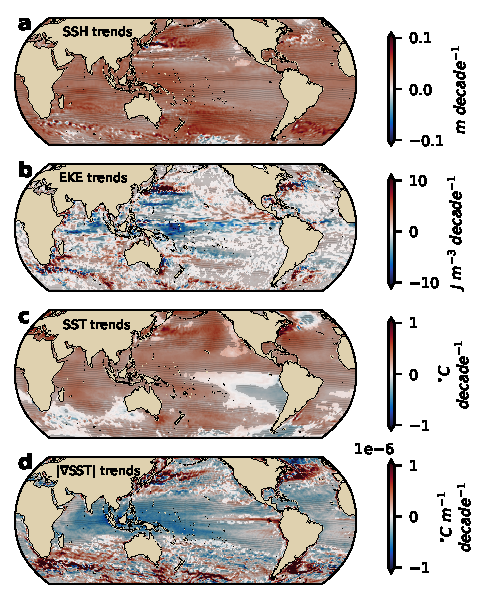
\includegraphics[width=0.8\textwidth]{./figures/global_SST_SST_grad_SSH_trends_signif.pdf}
	\caption{\textbf{Regions of statistically significant trends of (a) sea surface height; (b) surface eddy kinetic energy; (c) sea surface temperature; (d) sea surface temperature gradient magnitude.} As per Figs. 1b, 1f, 2b, and 2f in main manuscript, but showing in gray stippling regions that are statistically significant above the 95\% confidence level. \label{fig:global_significance_trends}}
\end{figureS}


\begin{figureS}
    \centering
	\hspace{0.1\textwidth}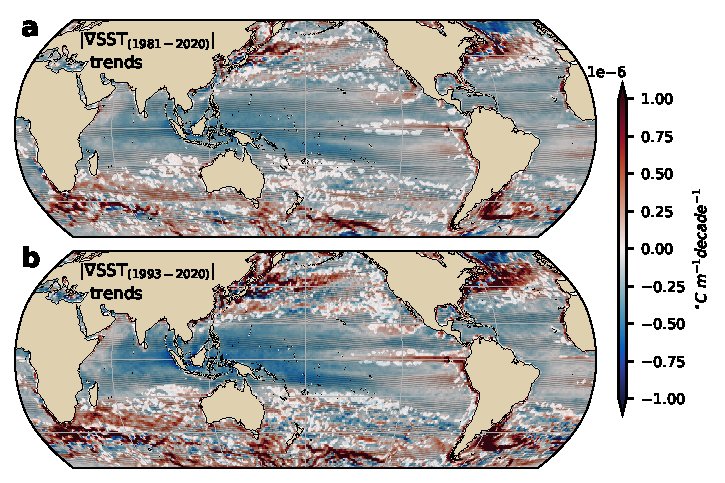
\includegraphics[width=0.8\textwidth]{./figures/global_SST_diff_time_records.pdf}
	\caption{\textbf{Sea surface temperature gradient magnitude trends for periods between 1981-2020 and 1993-2020.} Gray stippling shows regions that are statistically significant above the 95\% confidence level. \label{fig:global_significance_trends}}
\end{figureS}


\begin{figureS}
    \centering
	\hspace{0.05\textwidth}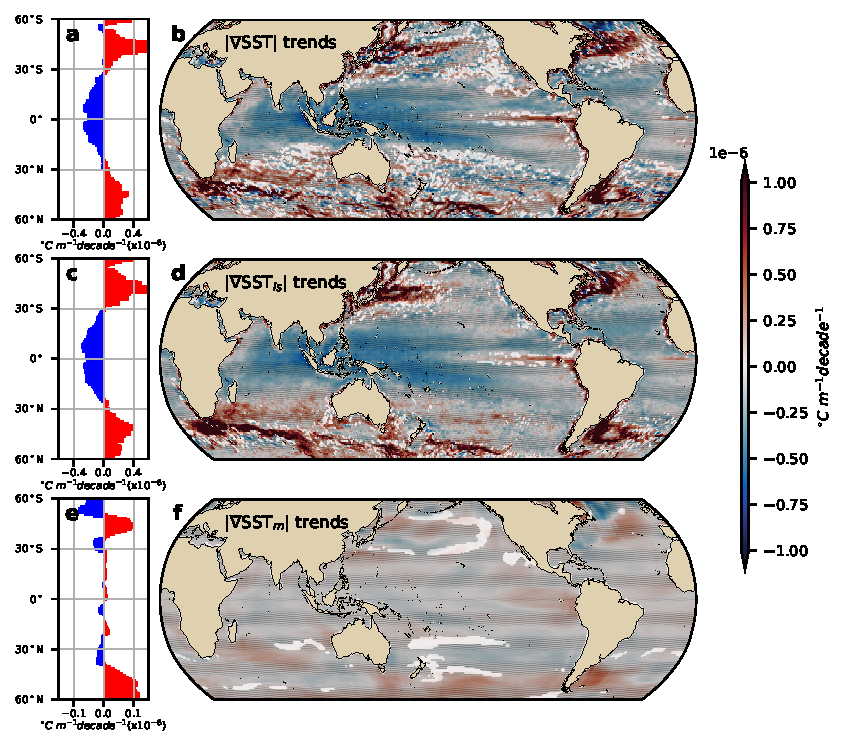
\includegraphics[width=0.9\textwidth]{./figures/global_SST_diff_scales_trends.pdf}
	\caption{\textbf{Sea surface temperature gradient magnitude trend scale analysis.} Large-scale $\SST$ gradient magnitudes are computed by filtering the $\SST$ field with a 3$^\circ$ kernel filter and a running average of 12 months before computing the gradient magnitudes and their respective trends (see Methods). The small scales correspond to the gradients of the $\SST$ minus the large-scale filtered $\SST$ field. (a) Zonally averaged $\SST$ gradient magnitude trends; (b) map of  $\SST$ gradient magnitude trends; (c) zonally averaged small-scale $\SST$ gradient magnitude trends; (d) map of small-scale $\SST$ gradient magnitude trends; (e) zonally averaged large-scale $\SST$ gradient magnitude trends; (f) map of large-scale $\SST$ gradient magnitude trends. In panels (b), (d) and (f) gray stippling shows regions where the trends are statistically significant above the 95\% confidence level. \label{fig:global_SST_grad_scales}}
\end{figureS}

\begin{figureS}
    \centering
	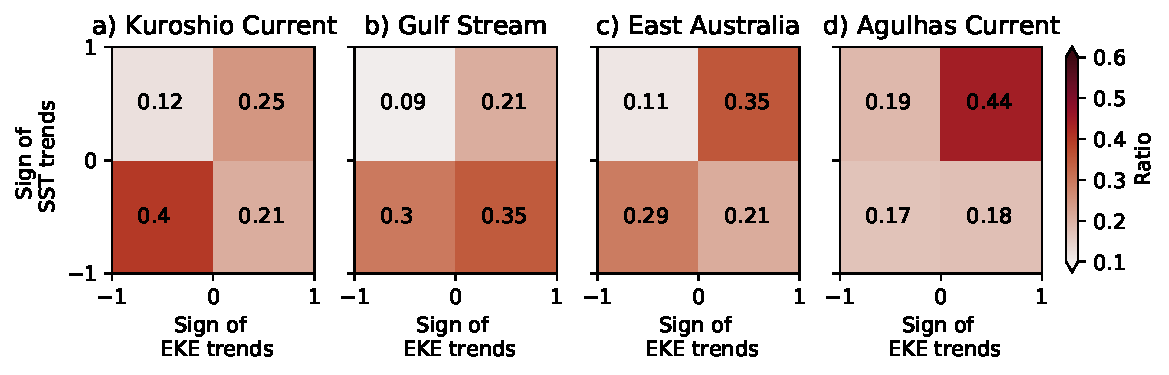
\includegraphics[width=1\textwidth]{./figures/trends_sign_correlations.pdf}
	\caption{\textbf{Regional ratio of mesoscale $\SST$ gradient magnitude trends and surface $\EKE$ trends signs}. (a) Kuroshio current; (b) Gulf Stream; (c) East Australian Current; (d) Agulhas retroflection. The ratio was computed by integrating the area weighted sign of the $\SST$ gradient magnitude trends and surface $\EKE$ trends divided by the total area of the region plotted in the Fig.~\ref{fig:WBC_regional_small_scale_SST_grad}. Quadrants I and III of each panel show colocated regions with the same sign in $\SST$ gradients and $\EKE$ trends, more than 60\% of the signs in the (a) Kuroshio current, (c) East Australian Current, and (d) Agulhas retroflection are colocated. \label{fig:trends_sign_correlations}}
\end{figureS}

\begin{figureS}
    \centering
	\hspace{0.1\textwidth}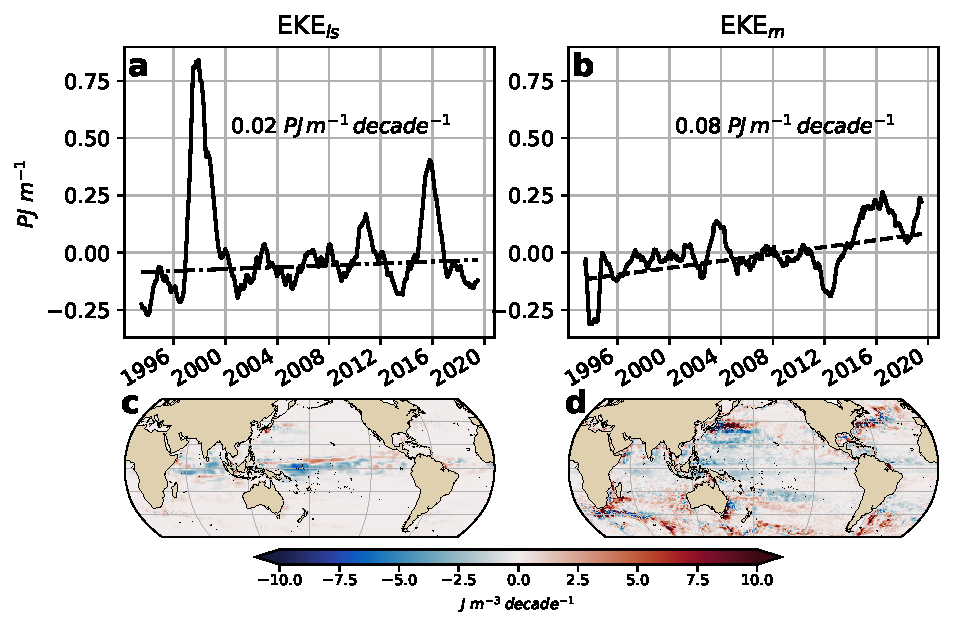
\includegraphics[width=0.8\textwidth]{./figures/large_scale_vs_small_scalle_eke.pdf}
	\caption{\textbf{Surface eddy kinetic energy time-series and trends computed from filtered velocities.} Scales larger than typical mesoscale are computed by filtering the surface velocity fields with a 3$^\circ$ kernel filter ($u_{ls}$), and the smaller scales are calculated from the difference of the velocity fields and the filtered velocity field ($u_e = u - u_{ls}$). Then surface $\EKE$ and their respective trends are computed (see Methods). (a) $\EKE$ time series of scales larger than 3 degrees time series; (b) $\EKE$ time series of scales smaller than 3 degrees; (c) map of large-scale $\EKE$ trends; (d) map of small-scale $\EKE$ trends. Text in panels (a) and (b) correspond to trends per decade.\label{fig:mesoscale_decomposition_eke}}
\end{figureS}

\begin{figureS}
    \centering
	\hspace{0.05\textwidth}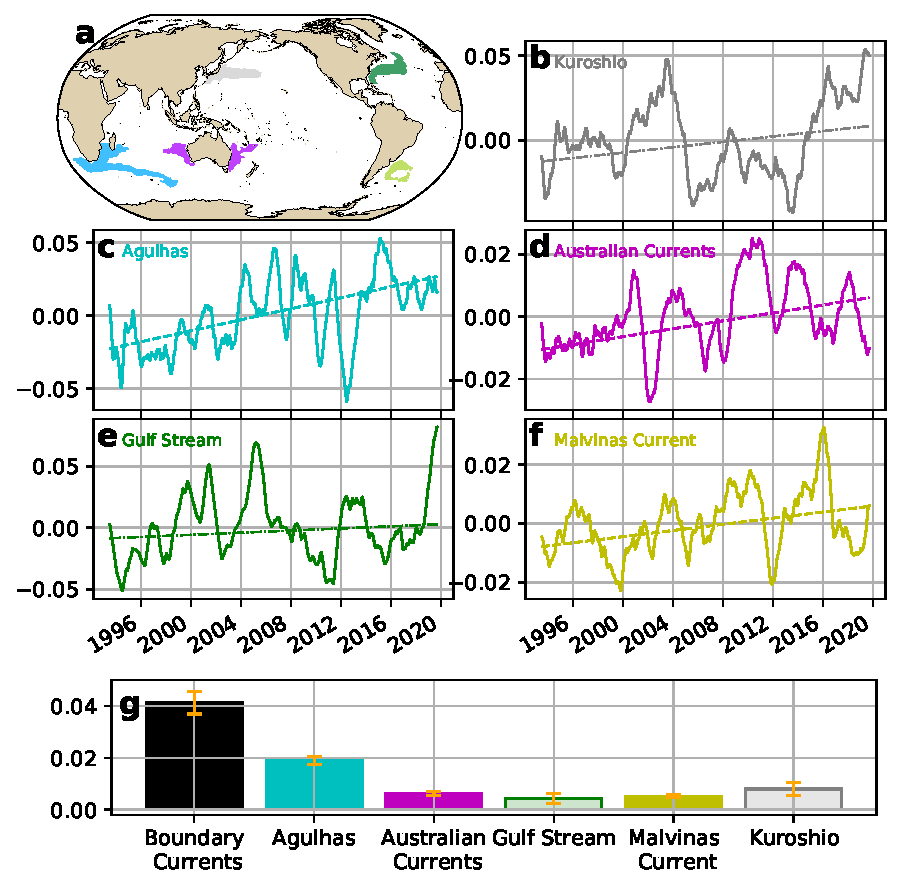
\includegraphics[width=0.9\textwidth]{./figures/global_wbc_decomposition_trends.pdf}
	\caption{\textbf{Time-series and trends of surface eddy kinetic energy integrated over boundary currents.} (a) Map of boundary current regions defined from climatological mean $\EKE$ and time series anomalies ($PJ\ m^{-1}$) and trends ($PJ\ m^{-1}\ decade^{-1}$) for each boundary current : (b) Kuroshio Current; (c) Agulhas Current; (d) East Australian Current and Leeuwin Current; (e) Gulf Stream; (f) Malvinas Current. (g) Linear $\EKE$ trends for boundary currents, uncertainties are shown in orange bars and statistically significant trends (above the 95\% confidence level) are denoted with solid bars while non-significant trends are translucent.\label{fig:individual_boundary_currents}}
\end{figureS}

\begin{figureS}
	\centering
    \hspace{0.075\textwidth}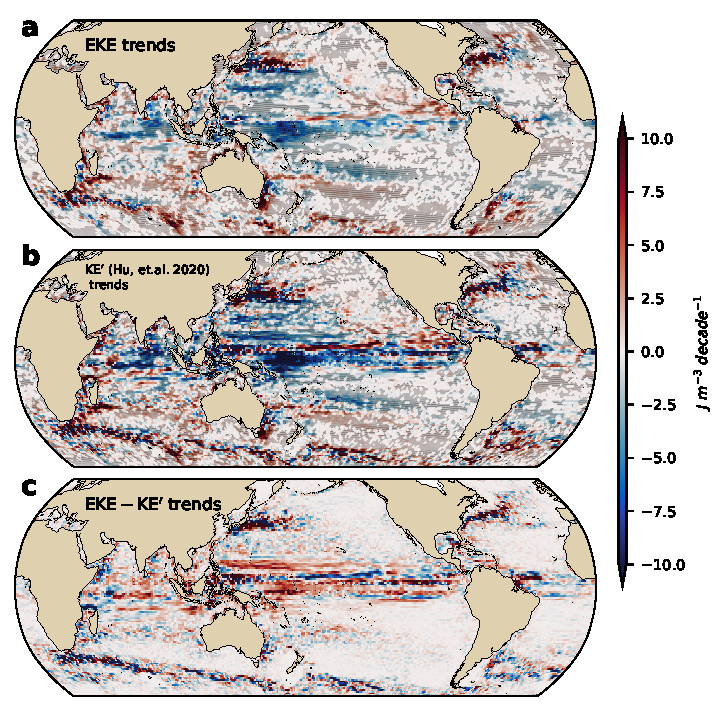
\includegraphics[width=0.85\textwidth]{./figures/global_trend_hu_comparison.pdf}
	\caption{\textbf{Comparison of satellite trends using surface $\EKE$ and kinetic energy anomaly ($\KE$') as computed by Hu et al., 2020 \cite{Hu_acceleration_2020}} (a) $\EKE$ trend map, (b) $\KE'$ trend map, and (c) difference between $\EKE$  and $\KE'$ trends. The difference between the fields is a consequence of the cross terms due to the Reynolds velocity decomposition. In panel (a) and (b) gray stippling shows regions where the trends are statistically significant above the 95\% confidence level. \label{fig:global_trends_asper_hu}}
\end{figureS}

\end{document}